%%%%%%%%%%%%%%%%%%%%%%%%%%%%%%%%%%%%%%%%%%%%%%%%%%%%%%%%%%%%%%%%%
% Dissertacao de Mestrado / Dept Fisica, CFM, UFSC              %
% Lacerda@UFSC - 2013                                           %
%%%%%%%%%%%%%%%%%%%%%%%%%%%%%%%%%%%%%%%%%%%%%%%%%%%%%%%%%%%%%%%%%

%:::::::::::::::::::::::::::::::::::::::::::::::::::::::::::::::%
%                                                               %
%                          Capítulo 2                           %
%                                                               %
%:::::::::::::::::::::::::::::::::::::::::::::::::::::::::::::::%

%***************************************************************%
%                                                               %
%                      CALIFA & PyCASSO                         %
%                                                               %
%***************************************************************%

\chapter{O projeto CALIFA e os {\em pipelines} QBICK e PyCASSO}
\label{sec:CALePyC}

Nesse cenário de crescimento exponencial na quantidade de dados alavancados por novas tecnologias surge o CALIFA: um
projeto de IFS que está modificando nossa maneira de ver e pensar as galáxias no nosso universo. A beleza da
espectroscopia de campo integral é poder unir imageamento e espectroscopia, obtendo-se assim a galáxia vista como um
cubo de dados $(x, y, \lambda)$; para cada $\lambda$ temos uma imagem, e para cada par de ascenção reta e declinação
$(x, y)$ temos um espectro. Na primeira seção deste capítulo iremos apresentar o survey CALIFA, que possibilita que este
trabalho seja pioneiro na execução de análise PCA em cubos de espectros abrangendo o campo de uma galáxia completa.

Com a enorme quantidade de dados obtidos, resultado direto de um projeto de ciência de ponta, vem também a dificuldade
da organização dos dados para futuras investigações científicas. Dois {\em pipelines} nos ajudam na preparação dos dados
que iremos usar neste trabalho, {\sc qbick} e PyCASSO. O {\sc qbick} prepara os dados para a síntese de populações
estelares e o PyCASSO organiza a saída da síntese, que é executada para cada espectro dentro da galáxia. Na segunda
seção apresentaremos ambos, mostrando as peculiaridades e técnicas empregadas sobre os dados através do {\sc qbick} e da
descrição e alguns exemplos de utilização do PyCASSO.

%***************************************************************%
%                                                               %
%                            CALIFA                             %
%                                                               %
%***************************************************************%

\section{O survey CALIFA}
\label{sec:CALePyC:Apresent}

No sul da Espanha, mais precisamente em {\em Sierra de Los Filabres} (Andalucía), está situado Observatório Astronômico
Hispano-Alemão de {\em Calar Alto}. O projeto CALIFA está sendo possível através de observações pelo maior de seus 3
telescópios (3.5m) ao longo de 250 noites. Em comparação com o \SDSS, o CALIFA terá a mesma ordem de número de
espectros para estudo ($\sim 10^6$), mas, apesar de um número muito menor de galáxias, graças ao IFU será o com melhor
completeza por objeto. Existem alguns poucos surveys IFU e todos com, além de poucos objetos e {\em FoV} menor, focos de
estudo mais estreitos, dificultando o legado do survey para outras pequisas científicas mais abrangentes \citep[SAURON;
][região central de 72 galáxias com $z < 0.01$.]{de-Zeeuw2002} \citep[PINGS; ][algumas galáxias muito próximas ($\sim
10$ Mpc) e o estudo atual de 70 (U)LIRGs com $z <0.26$]{RosalesOrtega2010} \citep[VENGA; ][$30$ galáxias
espirais]{Blanc2010}. O CALIFA foi concebido para que seu legado seja abrangente, possibilitando diversos tipos de
estudos em diversas áreas. Outros surveys IFU ainda estão por vir, como SAMI \citep{Croom2012} e
MaNGA\footnote{\url{http://www.sdss3.org/future/manga.php}}

A amostra-mãe do projeto contém 939 galáxias (das quais $\sim 600$ serão observadas) com {\em redshifts} entre $0.005 <
z < 0.03$ que distribuídas cobrem o diagrama cor-magnitude com $M_r < -18$ (Figura \ref{fig:cm-uzMz}) em uma ampla
variedade de tipos morfologicos, massa em estrelas, condições do gás ionizado. Para melhor aproveitar o {\em FoV} do
instrumento de IFU é feito também um corte em dimensão ($\sim1^{\prime}$ em diâmetro). No telescópio usado para o
projeto está instalado o equipamento Potsdam Multi Aperture Spectrograph \citep[PMAS; ][]{Roth2005} no modo PPAK
\citep{Verheijen2004, Kelz2006} formando um espectrofotômetro de campo integrado com um {\em bundle} de 382 fibras
(Figura \ref{fig:BundlePPAK}), das quais, 331 são para observação dos objetos, outras 36 que fazem amostras para a
sutração do céu e outras 15 para calibração. Cada uma das {\em science fibers} (331) possui $2.7^{\prime\prime}$ de
diâmetro, formando um campo de visão hexagonal de $74^{\prime\prime} \times 64^{\prime\prime}$ ($\sim1.3$ arcmin$^2$)
que, através de uma técnica de três pontos de {\em dithering} torna possível a observação de 100\% do campo.

\begin{figure}
    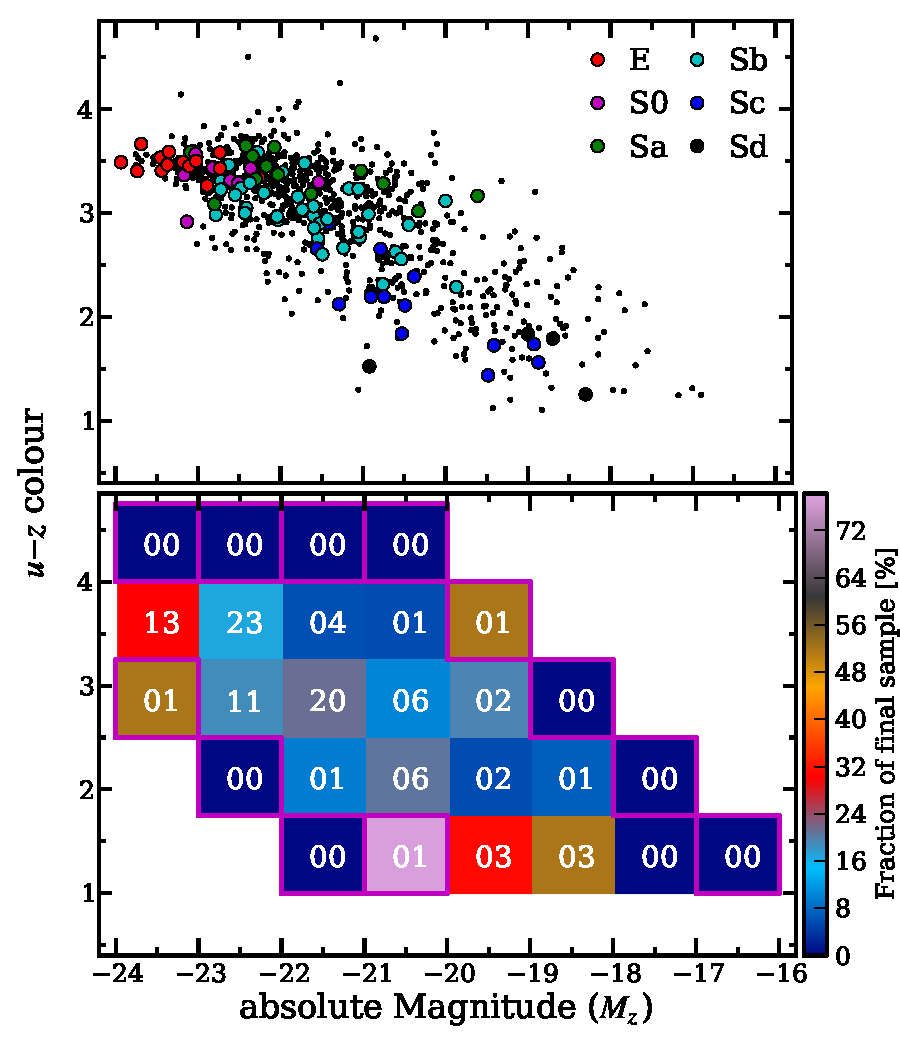
\includegraphics[height=0.5\textwidth]{figuras/figHusemann2013Fig2.pdf}
    \caption[Diagrama cor-magnitude para as galáxias do CALIFA.]
    {Distribui\c{c}\~ao das galáxias do CALIFA no diagrama cor magnitude $u-z$ vs. $M_z$. {\em Painel superior}: Em
    pontos pretos est\~ao as galáxias pertencente a amostra-m\~ae e em cores as galáxias presentes no CALIFA DR1. As
    diferentes cores representam os diferentes tipos morfológicos. {\em Painel inferor}: A fra\c{c}\~ao de galáxias
    observadas pelo DR1 em rela\c{c}\~ao a amostra-m\~ae. Retirado de \citet{Husemann2013}.}
    \label{fig:cm-uzMz}
\end{figure}

\begin{figure}
    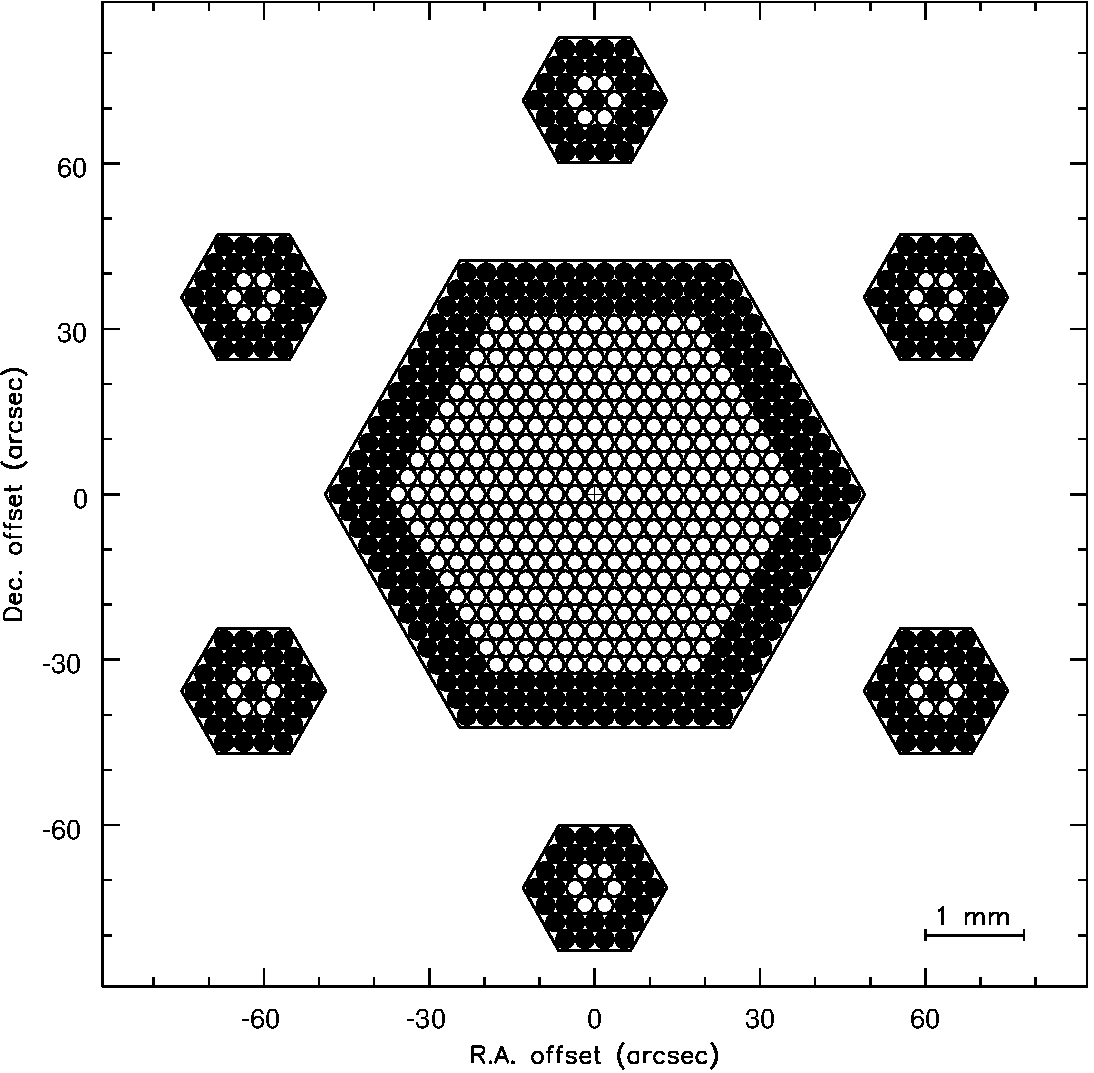
\includegraphics[height=0.5\textwidth]{figuras/figVerheijen2004Fig5.pdf}
    \caption[Configura\c{c}\~ao do {\em bundle} de fibras do PPMAS/PPAK.]
    {Este é o esquema com o {\em bundle} hexagonal com as 331 fibras de observação e mais 36 de amostra de céu. Retirado
    de \citet{Verheijen2004}.}
    \label{fig:BundlePPAK}
\end{figure}

Os dados são reduzidos utilizando o CALIFA Pipeline versão 1.3c, descrito em \citet{Husemann2013}. Com as 331 {\em
science fibers} e o processo de {\em dithering} em 3 posições, temos 993 espectros independentes por objeto observado.
\citet{Husemann2013} estimam que a resolução espacial final é $\sim3.7^{\prime\prime}$ (FWHM). Com a reamostragem do
cubo de espectros de forma que cada spaxel tenha área de $1^{\prime\prime} \times 1^{\prime\prime}$ obtêm-se mais de
4000 espectros por galáxia. Isto, somado ao {\em seeing} do céu e o processo de observação e redução, implica que cada
píxel do cubo final não seja completamente independente, ou seja, numa automática correlação entre os pixels vizinhos.
Os espectros vêm em duas configurações de rede: a V500 cobrindo de $\sim 3700$ até 7000 \AA\ com resolução de $\sim 6$
\AA\ de largura à meia altura (FWHM) e a V1200 ($\sim 3650-4600$ \AA\ FWHM $\sim2.3$ \AA). A cobertura espectral da
V$500$ é ideal para os propósitos de ciência feita pelo \starlight, mas por problemas com {\em vignetting} com a parte
azul dessa configuração, os dados são reamostrados numa combinação das duas redes, criando cubos que chamamos de COMBO:
A parte com $\lambda < 4600$ \AA\ vem da V1200 e o resto da V500. Nessa montagem os espectros da V1200 foram suavizados
à mesma resolução espectral da V500 (FWHM $= 6$ \AA). Como outros cubos do CALIFA, os cubos COMBO provêm, para cada
posição e comprimento de onda, o fluxo ($F_{\lambda,x,y}^{orig}$), seu erro ($\epsilon_{\lambda,x,y}$) e uma flag
($b_{\lambda,x,y}$) que sinaliza pixels defeituosos.

Nesse trabalho usaremos exclusivamente dados dos cubos COMBO. Por alguns motivos que veremos na próxima seção não
analisarermos exatamente esses dados em sua forma original, mas os provenientes de dois outros {\em pipelines}
desenvolvidas por nossa equipe.

%***************************************************************%
%                                                               %
%                            PyCASSO                            %
%                                                               %
%***************************************************************%

\section{Os {\em pipelines} QBICK e PyCASSO}
\label{sec:CALePyC:pipelines}

Em CF13 temos a descrição de duas pipelines usadas na análise dos cubos COMBO: O {\sc qbick} e o PyCASSO. Abaixo
revisamos esses pipelines, ambas muito importantes nesse trabalho.

\subsection{QBICK}

O primeira é o {\sc qbick}, desenvolvido por Rubén García-Benito, do IAA, e explicado em detalhe em CF13. Resumidamente,
este pipeline:

\begin{enumerate}
\item Cria máscaras espaciais que removem regiões externas de baixo S/N, e objetos indesejáveis no {\em FoV} (estrelas
ou galáxias).
\item Introduz flags espectrais que indicam janelas contendo linhas telúricas, cuja remoção imperfeita pode afetar os
espectros das regiões de menor fluxo.
\item Desloca o espectro para o referencial de repouso (usando o {\em redshift} calculado dentro dos $5^{\prime\prime}$
centrais da galáxia) e o reamostra a 2 \AA.
\item Define zonas de Voronoi, tal que o espectro total dessas zonas tem uma relação S/N $\ge 20$ em uma janela
espectral de 90 \AA\ de largura e centrada em 5635 \AA, e, por fim, extrai os espectros correspondentes.
\end{enumerate}

\begin{figure}
    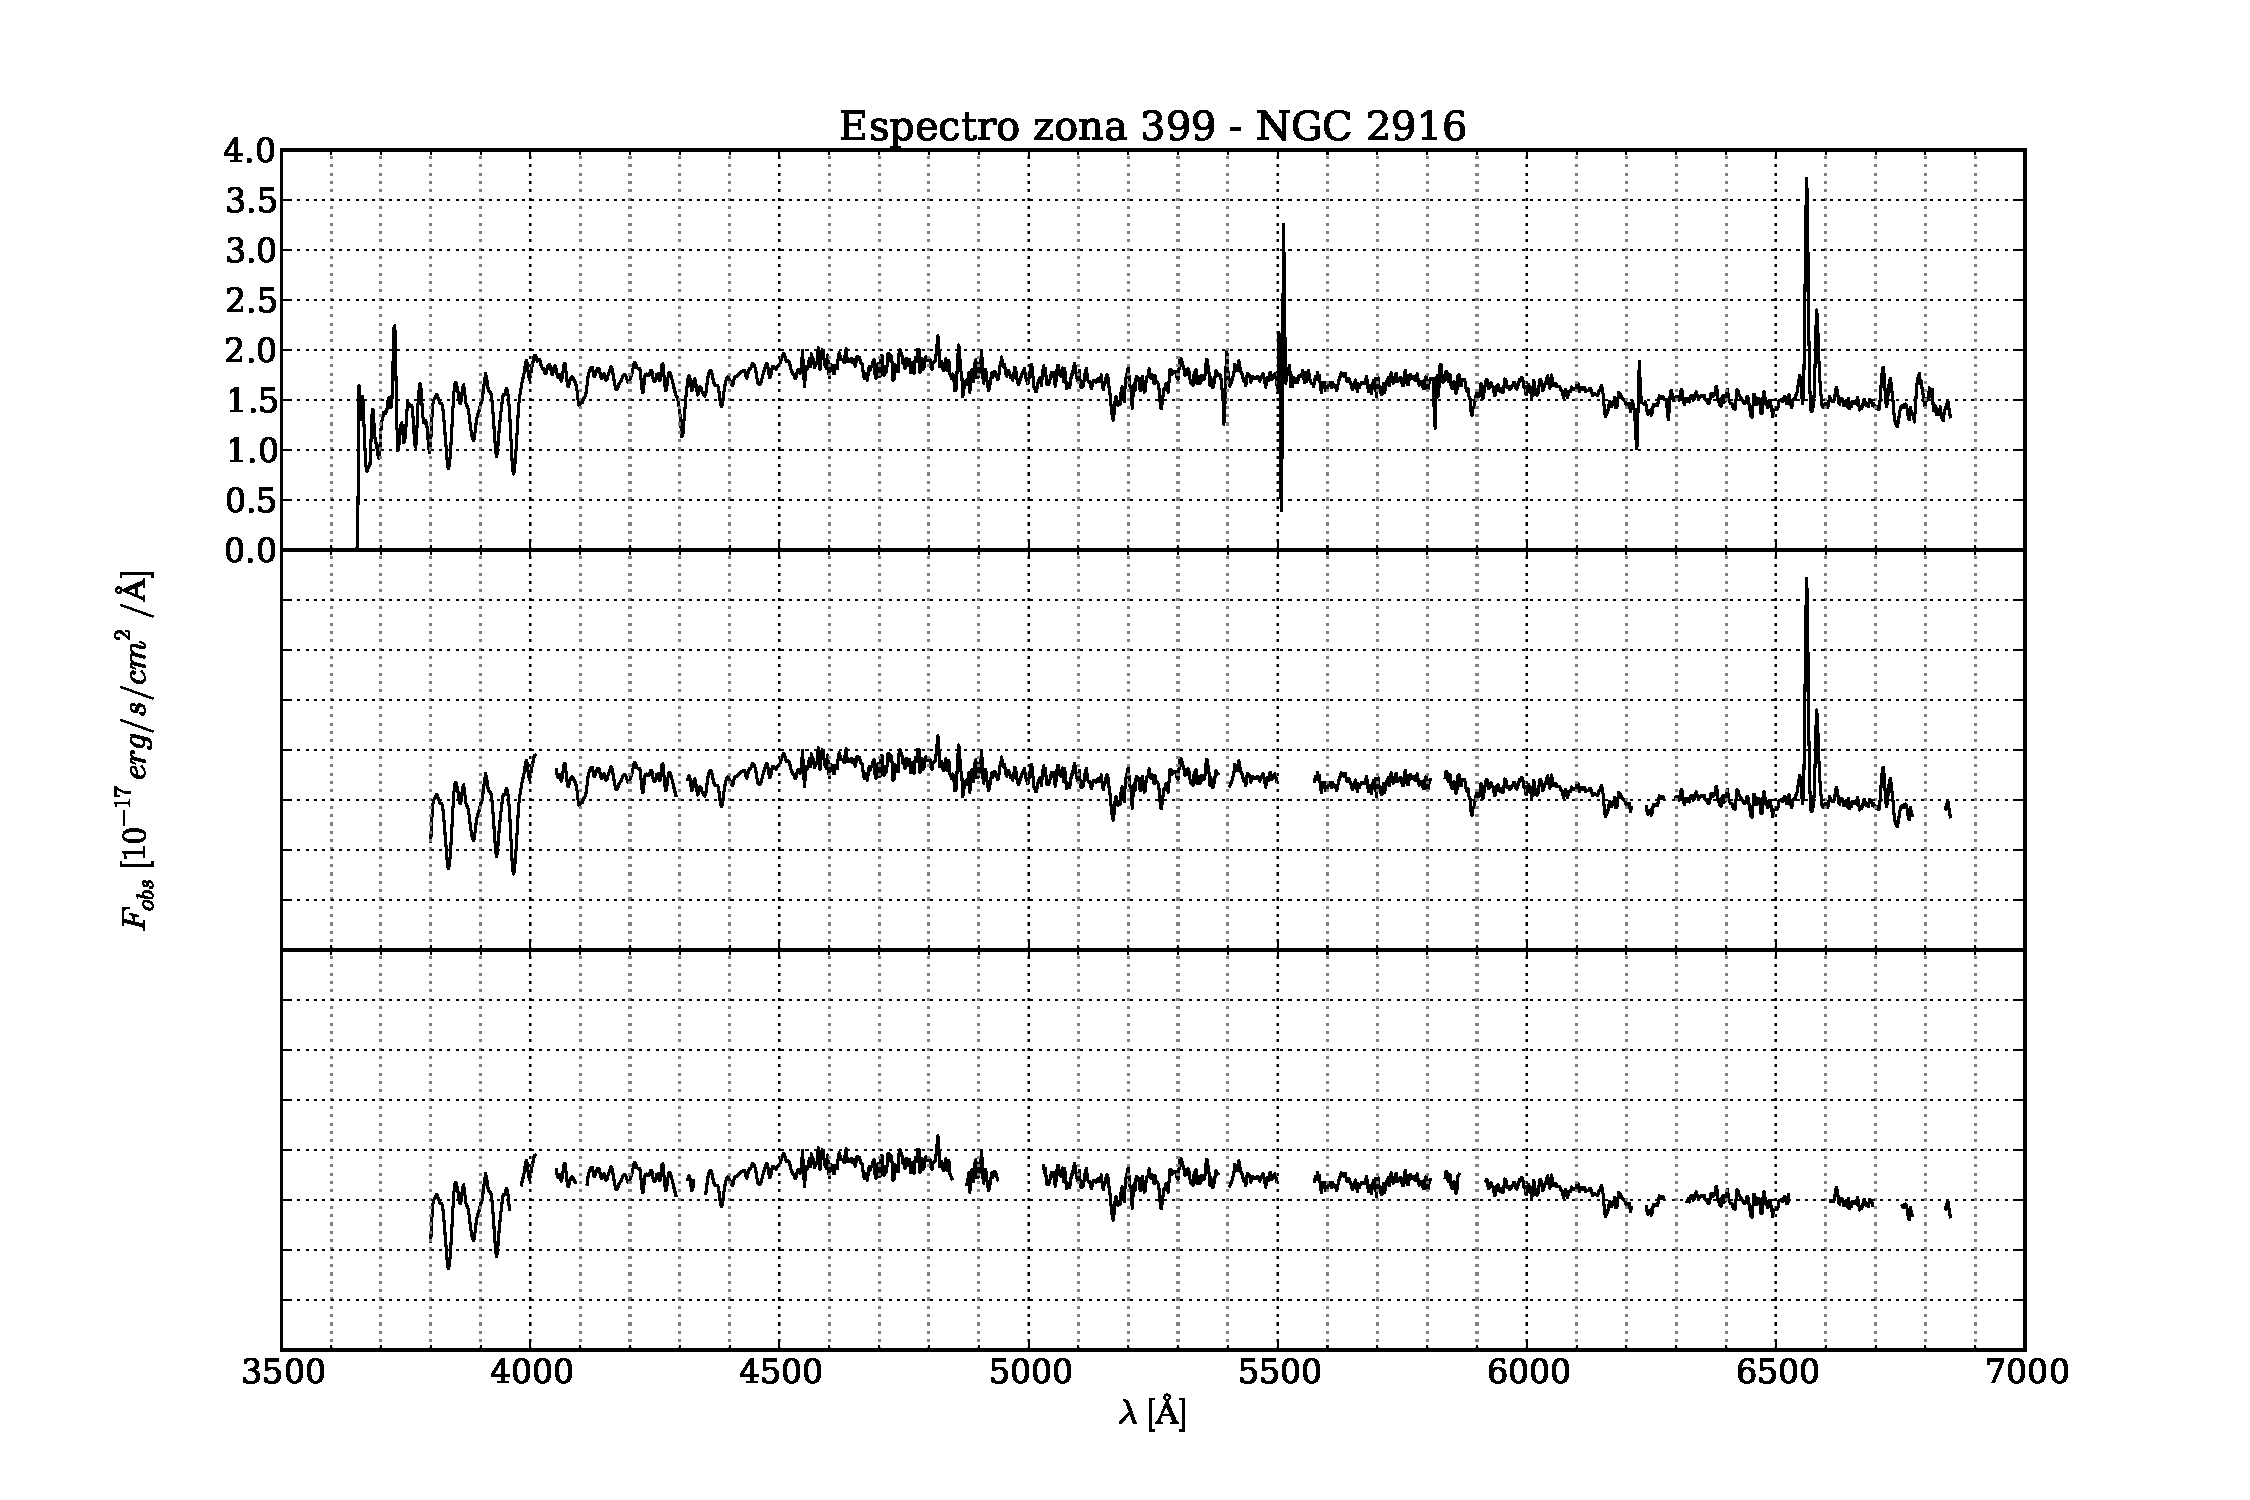
\includegraphics[width=1.0\textwidth]{figuras/K0277-constant_inital_mask-399.pdf}
    \caption[Exemplo de máscaras em um espectro do cubo de dados.]
    {Espectro da zona 399 da galáxia NGC 2916 (CALIFA 277). Acima está o espectro completo. No segundo vemos o espectro
    com linhas telúricas e bad-pixels removidos, além do limite de intervalo em comprimendo de onda de $3800$ a $6850$
    \AA. No espectro mais abaixo, além das partes removidas no segundo, estão foram removidas também as mesmas linhas de
    emissão mascaradas na síntese de populações estelares.}
    \label{fig:checkmask}
\end{figure}

A Figura \ref{fig:checkmask} ilustra as máscaras espectrais utilizadas, tomando como exemplo a zona 399 para a galáxia
NGC 2916 (CALIFA 277). O painel superior mostra o espectro original. No painel do meio as janelas mascaradas pelo {\sc
qbick} são removidas do espectro. Essas janelas correspondem a regiões contendo linhas telúricas\footnote{Linhas de
emissão ou absorção referentes à atmosfera.}, as quais dificilmente são perfeitamente removidas na redução. Pixels
identificados como problemáticos durante a redução dos dados são igualmente mascarados. Em nossa análise fazemos uma
estatística com todos os {\em bad pixels} de cada cubo e removemos qualquer um que esteja presente em mais de $5\%$ dos
espectros. Cabe aqui lembrar que todos os espectros precisam ter os mesmos pontos em comprimento de onda pois precisamos
construir a matriz de covariância (ver Equação \ref{eq:PCA:covMatrix}).
                                                                                                                                                                                                                                                                               
Além dos {\em bad pixels} e linhas telúricas, podemos mascarar regiões desnecessárias para determinada investigação
científica. Nosso foco é o estudo das populações estelares, e portanto optamos por mascarar as linhas de emissão.
Escolhemos mascarar as seguintes janelas: $\mathrm{H}\epsilon$: de 3960 a 3980 \AA; $\mathrm{H}\delta$: de 4092 a 4112
\AA; $\mathrm{H}\gamma$: de 4330 a 4350 \AA; \Hbeta: de 4848 a 4874 \AA; \oIII: de 4940 a 5028 \AA;
$\mathrm{He\,\textsc{i}}$ e $\mathrm{Na\,\textsc{i}\ D}$\footnote{Na {\sc i} D não é uma linha de emissão, mas
mascaramos esse dubleto porque ele pode conter uma componente de absorção devida a presença de gás neutro no meio
interestelar.}:de 5866 a 5916 \AA; \Halpha e \nII: de 6528 a 6608 \AA; $\mathrm{S\,\textsc{ii}}$: de 6696 a 6752 \AA.
Essas máscaras são na verdade introduzidas em uma etapa posterior ao {\sc qbick}, quando os espectros são procesados com
o \starlight. Também nessa etapa os espectros são cortados entre 3800 e 6850 \AA. O espectro após todas máscaras pode
ser visto no painel inferior da Figura \ref{fig:checkmask}.

\begin{figure}
	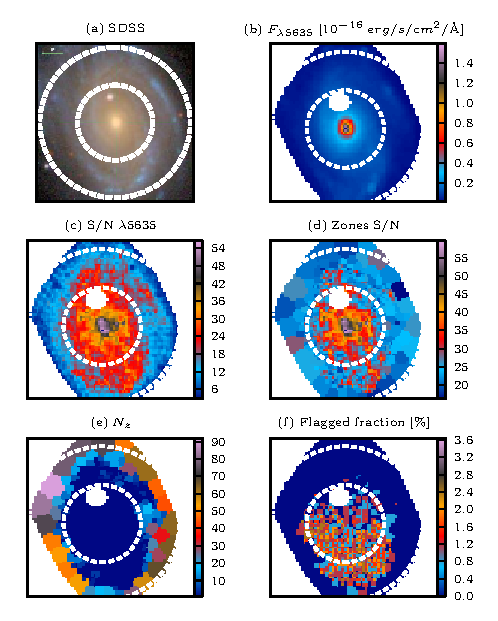
\includegraphics[width=1.0\textwidth]{figuras/figCF13fig1.pdf}
    \caption[Máscara espacial, zonas de Voronoi e flags para a galáxia NGC 2916 (CALIFA 277).]
    {(a) Imagem SDSS para a galáxia NGC 2916 (CALIFA 277). (b) Fluxo no intervalo de $5635 \pm 45$ \AA\ depois da
    aplicação da máscara espacial. (c) Mapa da relação S/N em 5635 \AA. (d) Mapa da relação S/N depois da zonificação de
    Voronoi. (e) Número de spaxels em cada zona de Voronoi. (f) Percentagem de {\em bad pixels} no intervalo
    de 3800--6850 \AA. Retirado de CF13, fig. 1.}
   	\label{fig:zonesfig1CF13}
\end{figure}

O efeito do agrupamento em zonas de Voronoi é ilustrado na Figura \ref{fig:zonesfig1CF13} para a galáxia NGC 2916 cujos
pixels úteis (i.e., não mascarados espacialmente) são agrupados em $N_z = 1638$ zonas. Como esperado, o efeito é maior
nas partes externas. Vale aqui frisar que a grande maioria das zonas comporta um pixel apenas. Para a galáxia NGC 2916,
por exemplo, $93\%$ das zonas possuem apenas 1 píxel e $\sim 3\%$ com mais de 10 pixels agrupados, mesmo com a imposição
de relaçao S/N $\ge 20$ na janela de $5635 \pm 45$ \AA, nossa janela de comprimento de onda usada como referência.
Podemos ver na Tabela \ref{tab:pixelZones} esses dados para as galáxias estudadas nesse trabalho. Portanto o cubo
original é transformado numa matriz de zonas e comprimentos de onda: $F_{zl}$ com $z = 1 \ldots N_z$ e $l = 3800 \ldots
6850$ \AA.

A motivação para a ``zonificação'' do cubo é garantir espectros de qualidade boa o suficiente para análise com o
\starlight. Nossa análise PCA poderia ser realizada sobre os cubos de dados originais, mas a realizaremos sobre as zonas
produzidas pelo {\sc qbick}. A razão para isso é que queremos comparar os resultados de nossa análise com os parâmetros
extraídos pelo \starlight, o que servirá de auxílio a interpretação dos resultados da PCA.

\begin{table}
	\caption[Relação de pixels e zonas em algumas galáxias do CALIFA.]
	{Relação entre números de pixels por zona nas galáxias do CALIFA utilizadas neste trabalho. $N_z$ representa o número
	de zonas. $N_1$ é o numero de zonas com $1$ pixel apenas e $N_{10}$ aquelas que possuem mais de $10$ pixels por zona.}
	\begin{tabular}{l l c r r r r r}
		Nome da galáxia & CALIFA ID & {\em Hubble Type} & $N_z$ & $N_{1}$ &
		${}^{N_1}/_{N_z}$ & $N_{10}$ & ${}^{N_{10}}/_{N_z}$
		\\
		\midrule
		NGC 0001 & K0008 & Sbc & $1132$ & $1077$ & $0.95$ & $40$ & $0.04$ \\
		NGC 0776 & K0073 & Sb  & $1733$ & $1628$ & $0.94$ & $61$ & $0.04$ \\
		NGC 1167 & K0119 & S0  & $1879$ & $1771$ & $0.94$ & $50$ & $0.03$ \\
		NGC 2623 & K0213 & Scd & $561$  & $530$  & $0.94$ & $19$ & $0.03$ \\
		NGC 2916 & K0277 & Sbc & $1638$ & $1528$ & $0.93$ & $53$ & $0.03$ \\
		NGC 4210 & K0518 & Sb  & $1938$ & $1847$ & $0.95$ & $38$ & $0.02$ \\
		ARP 220  & K0802 & Sd  & $1157$ & $1103$ & $0.95$ & $39$ & $0.03$ \\
		NGC 6515 & K0864 & E3  & $887$  & $811$  & $0.91$ & $44$ & $0.05$ \\
	\end{tabular}
	\label{tab:pixelZones}
\end{table}

Todas informações e pré-processamentos provenientes do {\sc qbick} são herdadas pelo {\em pipeline} apresentado a
seguir.

\subsection{PyCASSO}

Os espectros extraídos pelo {\sc qbick} são processados pelo \starlight, produzindo, no caso de CALIFA 277, 1639
arquivos ASCII como output. Dado o grande número de informações contidas em cada um desses arquivos (e.g., história de
formação estelar em luz e massa, extinção, parâmetros cinemáticos, figuras de mérito do ajuste), necessitamos de um
{\em pipeline} que faça a organização de todos os dados para que cálculos e gráficos sejam fácil para que até um programador
de nível iniciante possa fazer. André L. de Amorim, juntamente com outros colaboradores de nosso grupo e do projeto
CALIFA construiu o PyCASSO ({\em Python CALIFA \starlight Synthesis Organizer}) (descrito na sec. 4 de CF13) que faz a
organização dos dados que vêm do {\sc qbick} e das etapas inicais de redução juntamente com a síntese de populações
estelares feitas com o \starlight, facilitando, e muito, o trabalho de quem usa estes dados. Sem a ajuda deste
organizador, este trabalho seria muito mais difícil, além de infactível no tempo de um mestrado.

O PyCASSO é uma biblioteca desenvolvida em Python para organizar os dados da síntese feita pelo \starlight. A versão
usada neste trabalho é a $0.9.3$\footnote{\url{http://minerva.ufsc.br/~andre/PyCASSO-0.9.3/}}. Para um acesso mais
rápido e reutilizável do código e dos dados em qualquer ambiente, organiza os cubos em formatos FITS ou HDF5. Em outra
camada, várias matrizes e cubos são armazenados para acesso com nomes próprio (um exemplo, \texttt{popx}, representa a
fração de luz distribuída pelas populações estelares da base usada na síntese espectral com o \starlight) de forma que a
programação exploratória não precise se preocupar com as características de cada formato de armazenamento de dados. Por
fim, existe uma camada construída para análise, com funções que retornam a indexação de cada zona para um par $(x, y)$,
cálculos de perfis radiais e azimutais, geometria, entre outras rotinas. Um programador facilmente pode adicionar mais
rotinas como essas. Todos os códigos desenvolvidos nessa dissertação foram escritos de forma compatível com o PyCASSO.

\subsection{Exemplos de utilização do PyCASSO}

\begin{figure}
	\begin{python}
# Carregar arquivo FITS com os dados.
from pycasso import fitsQ3DataCube
K = fitsQ3DataCube('K0277_synthesis_suffix.fits')

# Acessar a idade media ponderada pela luminosidade.
at = K.at_flux__z

# Calcular a idade media da galaxia.
at_total = (at * K.Lobn__z).sum() / K.Lobn__z.sum()
print 'Idade media da galaxia K0277: \%.2f' \% at_total
	\end{python}
	\caption[Exemplo de programa utilizando PyCASSO.]
	{Exemplo de acesso aos cubo de dados por arquivo FITS e o cálculo da idade estelar média de uma galáxia.}
	\label{fig:dataAccess}
\end{figure}

\begin{figure}
	\begin{python}
# Carregar arquivo FITS com os dados.
from pycasso import fitsQ3DataCube
K = fitsQ3DataCube('K0277_synthesis_suffix.fits')

# Converter zonas para imagem.
at_image = K.zoneToYX(K.at_flux__z, extensive=False)

# Desenhar o mapa.
import matplotlib.pyplot as plt
plt.imshow(at_image, origin='lower', interpolation='nearest')
plt.xlabel('Pixels')
cb = plt.colorbar()
cb.set_label(r'\langle \log t \langle_L [anos]')
plt.title(r'\langle \log t \langle_{L z}')
	\end{python}
	\caption[Programa idade estelar média.]
	{Programa para desenhar o mapa de idade	estelar média ponderada pela luminosidade.}
	\label{fig:programaMapaIdade}
\end{figure}

\begin{figure}
	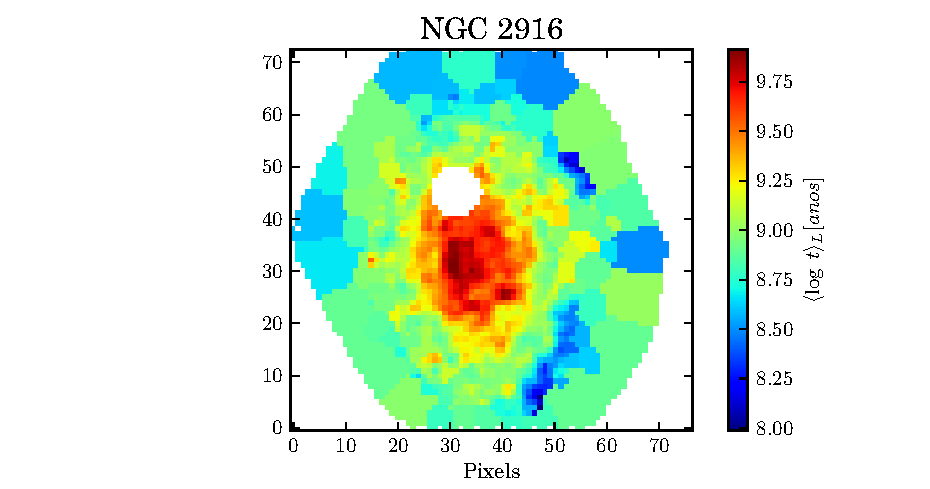
\includegraphics{figuras/at_flux_zone.pdf}
	\caption[Mapa da idade estelar média da galáxia NGC 2916 (CALIFA 277).] 
	{Mapa de idade estelar média ponderada pela luminosidade da galáxia NGC 2916 (CALIFA 277) gerado pelo programa da
	Figura \ref{fig:programaMapaIdade}.}
	\label{fig:mapaIdade}
\end{figure}

Ler um arquivo FITS é fácil com o PyCASSO, assim como o acesso aos dados. Na Figura \ref{fig:dataAccess} temos um
exemplo de leitura de arquivo FITS e um cálculo da idade estelar média da galáxia a partir da idade média ponderada pela
luminosidade, por zona (\texttt{at\_flux\_\_z}). A idade estelar média é calculada usando a expressão $ \langle \log t
\rangle^{gal}_L = \sum_z \langle \log t \rangle_{L,z} L_z /\sum_z L_z$ onde $L_Z $ é a luminosidade e $ \langle \log t
\rangle_L $ é a idade estelar média, ambas por zona. A passagem de coordenadas $z \to (x, y)$ exemplificada no programa
da Figura \ref{fig:programaMapaIdade} (e a imagem gerada na Figura \ref{fig:mapaIdade}) é feita através da função de
\texttt{zoneToYX} dentro do PyCASSO. Os gráficos são feitos utilizando a biblioteca gráfica de Python,
\texttt{matplotlib}\footnote{\url{http://matplotlib.org}}.

\begin{figure}
	\begin{python}
# Carregar arquivo FITS com os dados.
from pycasso import fitsQ3DataCube
K = fitsQ3DataCube('K0277_synthesis_suffix.fits')

# Converter zonas para imagem.
at_image = K.zoneToYX(K.at_flux__z, extensive=False)

# Calcular o perfil radial.
bins = np.arange(0, 26, 1)
bin_center = (bins[1:] + bins[:-1]) / 2.0
at_rad = K.radialProfile(at_imagem, bins, rad_scale = 1.0)

# Desenhar o perfil.
import matplotlib.pyplot as plt
plt.xlabel('radius [arcsec]')
plt.ylabel(r'\langle \log t \langle_L [anos]')
cb = plt.colorbar()
plt.plot(bin_center, at_rad)
	\end{python}
	\caption[Exemplo de programa para perfil radial.]
	{Programa para desenhar o perfil radial da idade estelar média ponderada pela
	luminosidade.}
	\label{fig:programaPerfRad}
\end{figure}

\begin{figure}
	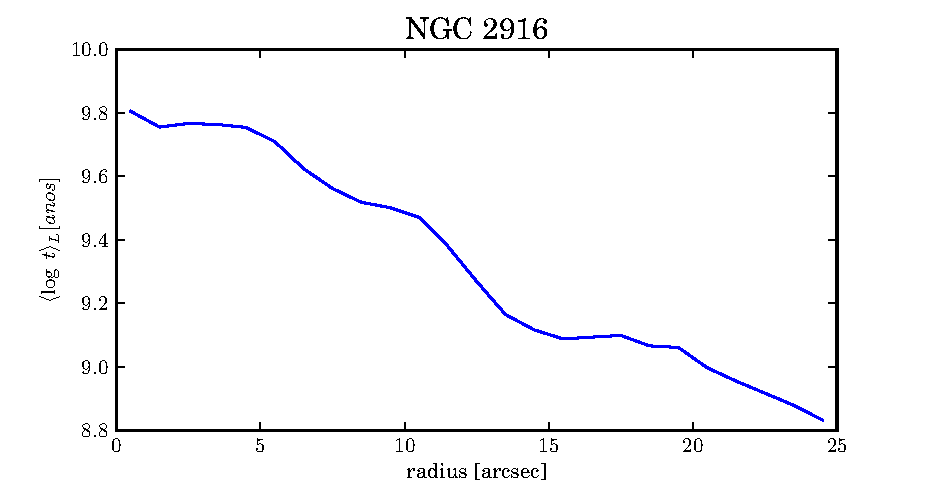
\includegraphics{figuras/at_flux_radprof.pdf}
	\caption[Perfil radial da idade estelar média da galáxia NGC 2916 (CALIFA 277).]
	{Perfil radial da idade estelar média ponderada pela luminosidade da galáxia
	NGC 2916 (CALIFA 277) gerado pelo programa da Figura \ref{fig:programaPerfRad}.}
	\label{fig:perfRad}
\end{figure}

Perfis radiais ou axiais também são importantes para o estudo de diversas propriedades galáticas. Podemos ver na Figura
\ref{fig:programaPerfRad} (e a imagem gerada na Figura \ref{fig:perfRad}) um exemplo de perfil radial executado
através da função \texttt{radialProfile} do PyCASSO.

Já existem vários artigos utilizando o PyCASSO \citep{CidFernandes2013, CidFernandes2014, Perez2013,
GonzalezDelgado2014}, também há alguns usando indiretamente \citep{Husemann2013, IglesiasParamo2013} e três teses de
doutorado em curso (uma na UFSC e duas no IAA). São mais de 10 pessoas utilizando a biblioteca em nossa colaboração. 

Os cálculos necessários para a PCA e também para a Tomografia PCA se tornam simples contas usando pacotes matemáticos de
python. O software dessenvolvido para a PCA e Tomografia PCA desta dissertação (por ora apelidado de ``PCAlifa'') foi
feito de forma compativel com o PyCASSO, visando futuramente integrá-lo como um novo módulo dessa ferramenta.

% End of this chapter
